\documentclass[tikz,border=8pt]{standalone}
\usepackage{tikz}
\usepackage{amssymb}
\usetikzlibrary{shapes.geometric, arrows.meta, positioning, calc, backgrounds, fit}

\definecolor{pbblue}{HTML}{E6F3FF}
\definecolor{pbdarkblue}{HTML}{1E3A8A}
\definecolor{pbmint}{HTML}{E0F2F1}
\definecolor{pbdarkgreen}{HTML}{065F46}
\definecolor{pblavender}{HTML}{F3E5F5}
\definecolor{pbdarkpurple}{HTML}{581C87}
\definecolor{pbyellow}{HTML}{FEF3C7}
\definecolor{pbdarkyellow}{HTML}{92400E}
\definecolor{pbcoral}{HTML}{FEE2E2}
\definecolor{pbdarkred}{HTML}{991B1B}
\definecolor{pbgray}{HTML}{F3F4F6}

\begin{document}
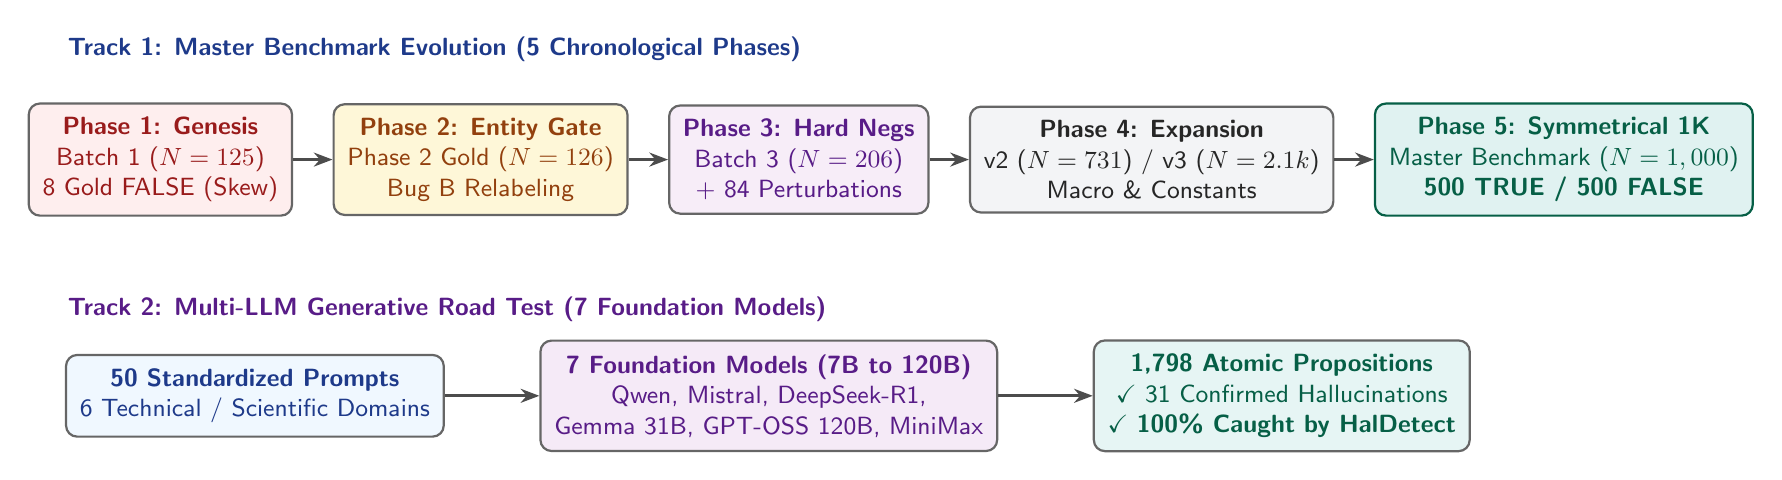
\begin{tikzpicture}[
    font=\sffamily\small,
    box/.style={draw=black!60, rounded corners=4pt, line width=0.8pt, align=center, inner sep=5pt},
    arrow/.style={-{Stealth[scale=0.9]}, line width=1.0pt, draw=black!70}
]

% ------------------- Track 1: 5-Phase Master Benchmark Evolution -------------------
\node[anchor=west, font=\bfseries\sffamily\small, text=pbdarkblue] at (0, 3.2) {Track 1: Master Benchmark Evolution (5 Chronological Phases)};

\node[box, fill=pbcoral!60, text=pbdarkred, minimum width=2.4cm] (p1) at (1.3, 1.8) {\textbf{Phase 1: Genesis}\\Batch 1 ($N=125$)\\8 Gold FALSE (Skew)};
\node[box, fill=pbyellow!70, text=pbdarkyellow, right=0.5cm of p1, minimum width=2.5cm] (p2) {\textbf{Phase 2: Entity Gate}\\Phase 2 Gold ($N=126$)\\Bug B Relabeling};
\node[box, fill=pblavender!70, text=pbdarkpurple, right=0.5cm of p2, minimum width=2.5cm] (p3) {\textbf{Phase 3: Hard Negs}\\Batch 3 ($N=206$)\\+ 84 Perturbations};
\node[box, fill=pbgray, text=black!85, right=0.5cm of p3, minimum width=2.5cm] (p4) {\textbf{Phase 4: Expansion}\\v2 ($N=731$) / v3 ($N=2.1\text{k}$)\\Macro \& Constants};
\node[box, fill=pbmint, draw=pbdarkgreen, text=pbdarkgreen, right=0.5cm of p4, minimum width=2.6cm] (p5) {\textbf{Phase 5: Symmetrical 1K}\\Master Benchmark ($N=1,000$)\\\textbf{500 TRUE / 500 FALSE}};

\draw[arrow] (p1) -- (p2);
\draw[arrow] (p2) -- (p3);
\draw[arrow] (p3) -- (p4);
\draw[arrow] (p4) -- (p5);

% ------------------- Track 2: Open Generative Road Test -------------------
\node[anchor=west, font=\bfseries\sffamily\small, text=pbdarkpurple] at (0, -0.1) {Track 2: Multi-LLM Generative Road Test (7 Foundation Models)};

\node[box, fill=pbblue!60, text=pbdarkblue, minimum width=3.6cm] (t2_prompts) at (2.5, -1.2) {\textbf{50 Standardized Prompts}\\6 Technical / Scientific Domains};
\node[box, fill=pblavender!80, text=pbdarkpurple, right=1.2cm of t2_prompts, minimum width=4.2cm] (t2_models) {\textbf{7 Foundation Models (7B to 120B)}\\Qwen, Mistral, DeepSeek-R1,\\Gemma 31B, GPT-OSS 120B, MiniMax};
\node[box, fill=pbmint!80, text=pbdarkgreen, right=1.2cm of t2_models, minimum width=3.8cm] (t2_props) {\textbf{1,798 Atomic Propositions}\\$\checkmark$ 31 Confirmed Hallucinations\\$\checkmark$ \textbf{100\% Caught by HalDetect}};

\draw[arrow] (t2_prompts) -- (t2_models);
\draw[arrow] (t2_models) -- (t2_props);

\end{tikzpicture}
\end{document}